\documentclass[]{article}
\usepackage{amsmath}
\usepackage{amsthm}
\usepackage{listings}
%\usepackage[margin=1.3cm]{geometry}
\usepackage{graphicx}
\usepackage{hyperref}

\title{Practical Lab Numerical Computing Computational Finance \\Bachelor-Worksheet 4}
\author{Lukas Troska, Ilja Kalmykov}
\date{}
\setlength{\parindent}{0pt}

\begin{document}

\maketitle

The referenced source code files can be found on
\url{https://github.com/iljaGH/CompFin/}.

\section*{Task 1}
\begin{figure}[!ht]
\centering
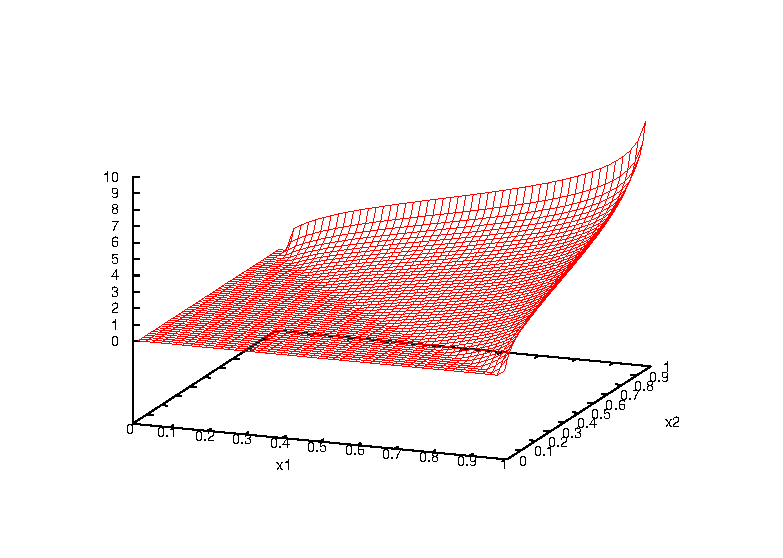
\includegraphics[width=.9\textwidth]{task1.eps}
\caption{Integrand of 2 dimensional Down-Out Call option $S(0)=10,K=10,B=8,T=1,\sigma=0.2,r=0.05$}
\label{fig:Task1}
\end{figure}
\clearpage


\section*{Task 2}
Below are the two convergence plots for MC and QMC respectively. The third plot is a pseudo-convergence plot of MC using a low precision reference value. We see that the plot stabilizes at a higher "error". Parameters: $M=128,S(0)=10,K=10,B=9,T=1,\sigma=0.2,r=0.05$.

\begin{figure}[!ht]
\centering
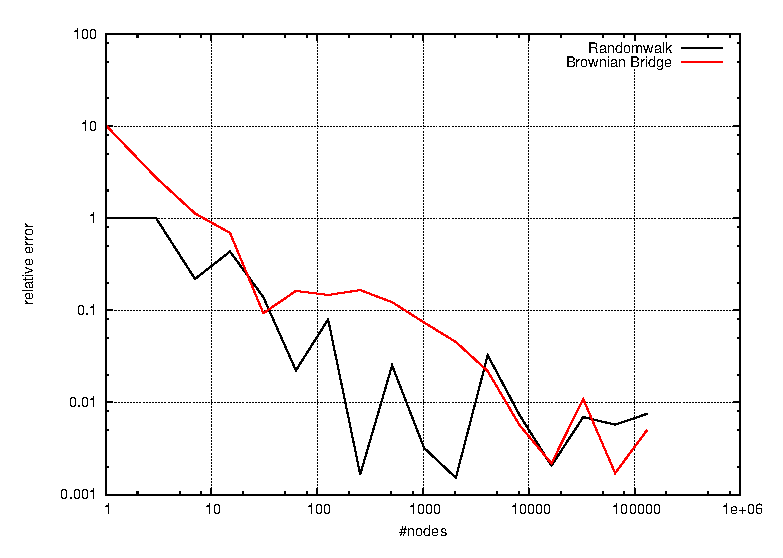
\includegraphics[width=.9\textwidth]{task2_mc_high.eps}
\caption{Monte-Carlo}
\label{fig:Task2a}
\end{figure}

\begin{figure}[!ht]
\centering
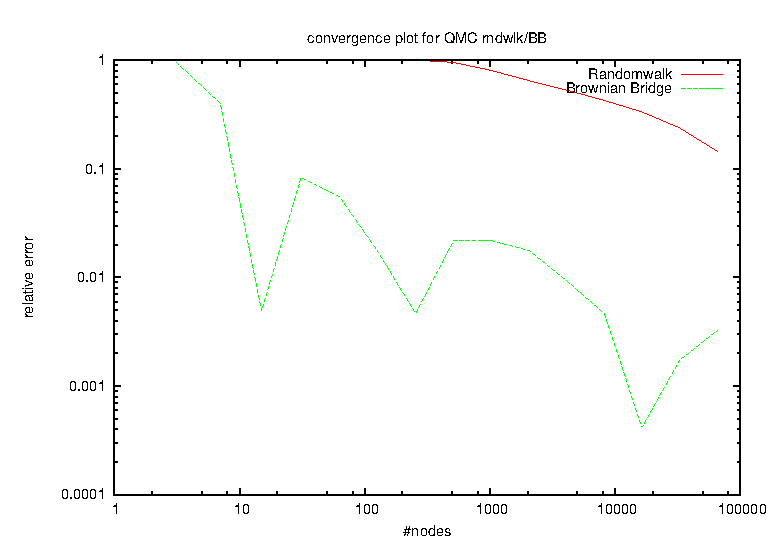
\includegraphics[width=.9\textwidth]{task2_qmc.eps}
\caption{Quasi-Monte-Carlo}
\label{fig:Task2b}
\end{figure}

\begin{figure}[!ht]
\centering
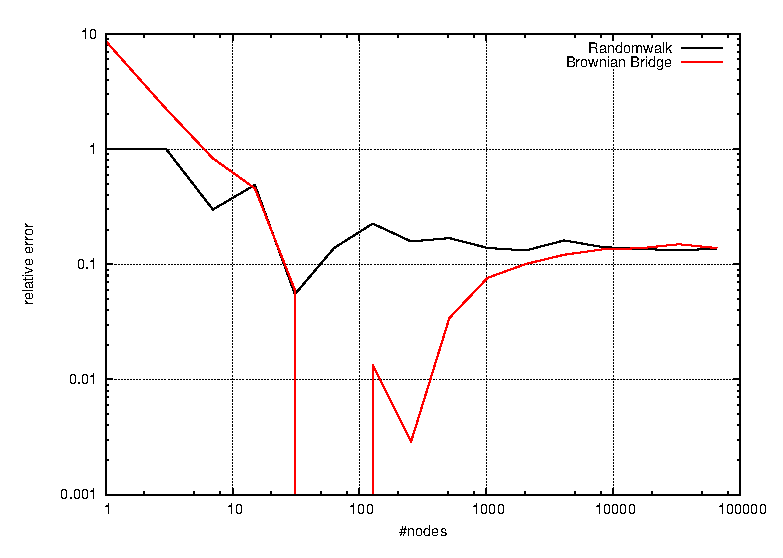
\includegraphics[width=.9\textwidth]{task2_mc_low.eps}
\caption{Monte-Carlo with low precision reference value}
\label{fig:Task2c}
\end{figure}
\clearpage

\section*{Task 3}
\begin{figure}[!ht]
\centering
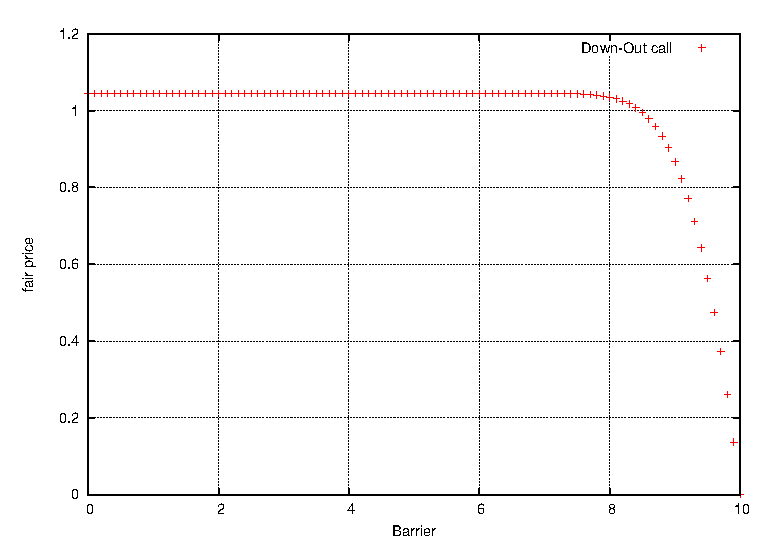
\includegraphics[width=.9\textwidth]{task3.eps}
\caption{fair price of Down-Out call options, parameters as above}
\label{fig:Task3}
\end{figure}
\clearpage


\section*{Task 4}
Parameters as above, convergence of Monte-Carlo Down-Out option.
\begin{figure}[!ht]
\centering
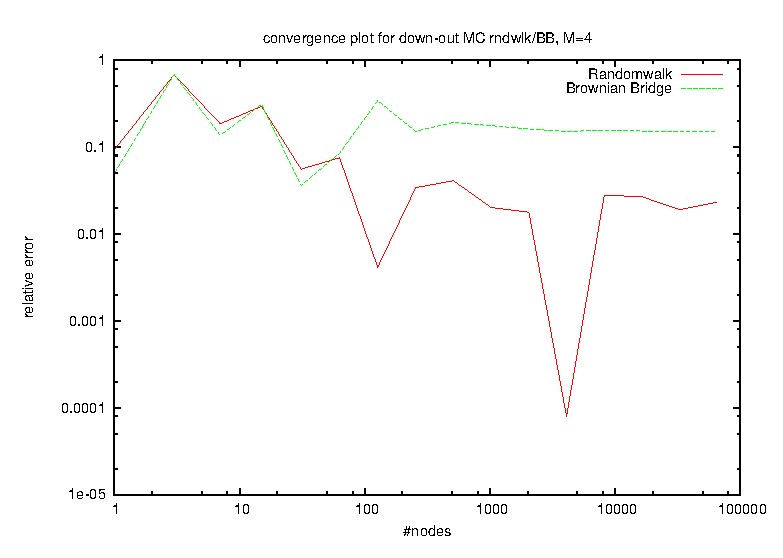
\includegraphics[width=.9\textwidth]{task4_mc_4.eps}
\caption{$M=4$}
\label{fig:Task4a}
\end{figure}

\begin{figure}[!ht]
\centering
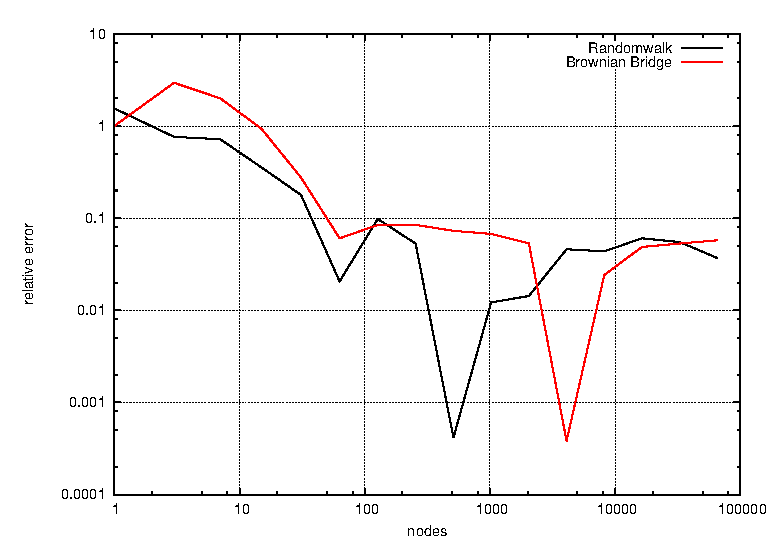
\includegraphics[width=.9\textwidth]{task4_mc_64.eps}
\caption{$M=64$}
\label{fig:Task4b}
\end{figure}

\begin{figure}[!ht]
\centering
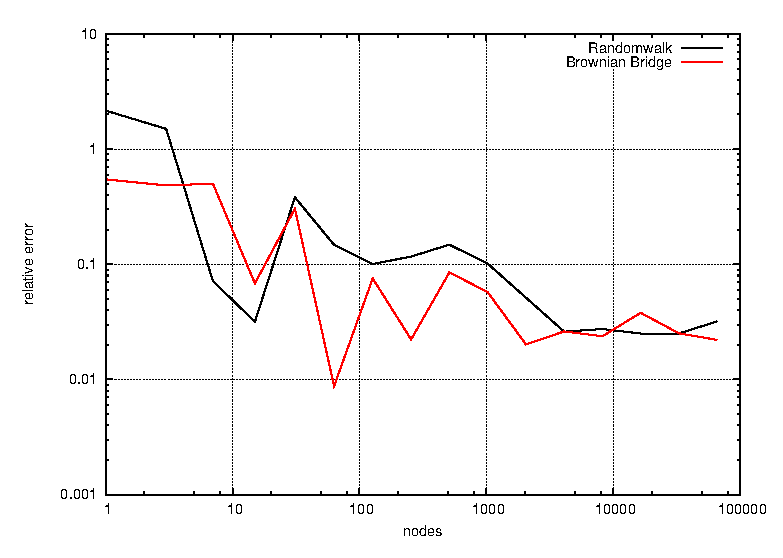
\includegraphics[width=.9\textwidth]{task4_mc_256.eps}
\caption{$M=256$}
\label{fig:Task4c}
\end{figure}

\begin{figure}[!ht]
\centering
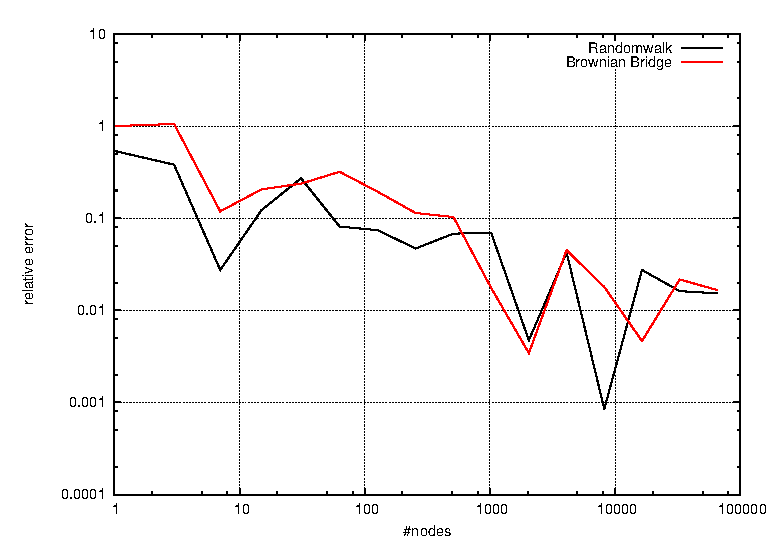
\includegraphics[width=.9\textwidth]{task4_mc_1024.eps}
\caption{$M=1024$}
\label{fig:Task4d}
\end{figure}
\clearpage

\section*{Task 5}
\begin{figure}[!ht]
\centering
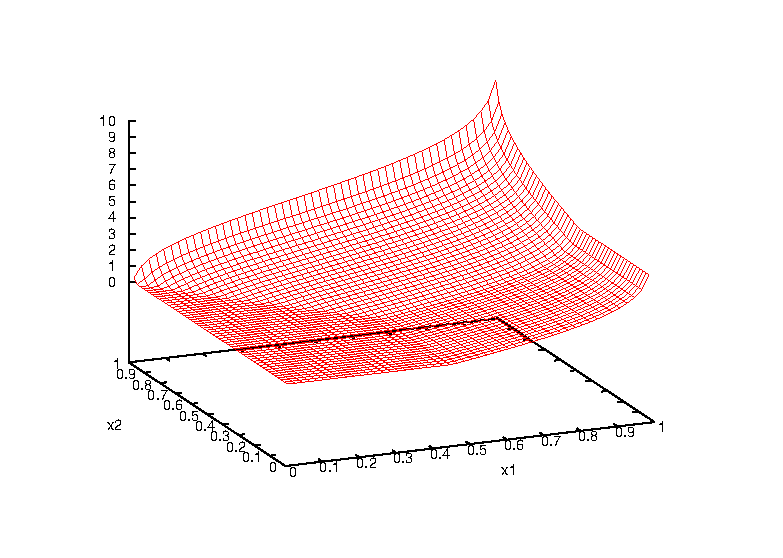
\includegraphics[width=.9\textwidth]{task5.eps}
\caption{Lookback option, discrete time integrand with parameters, $M=2,S(0)=10,K=10,T=1,\sigma=0.2,r=0.05$}
\label{fig:Task5}
\end{figure}
\clearpage

\section*{Task 6}
\begin{figure}[!ht]
\centering
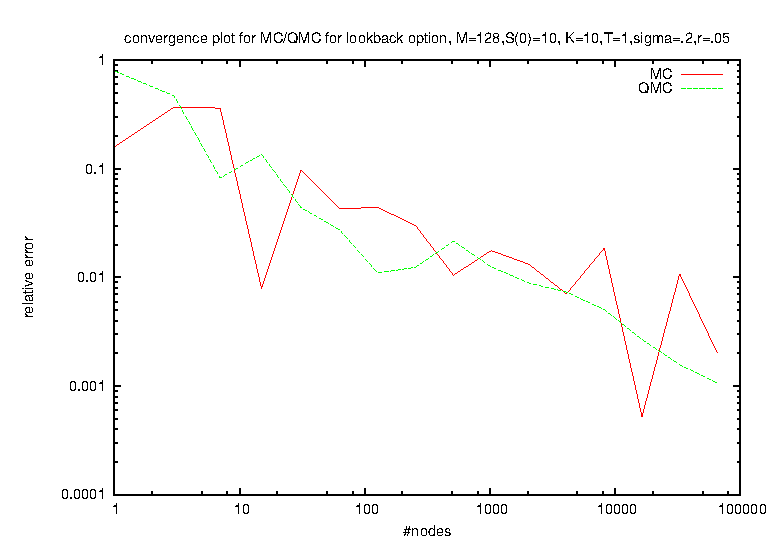
\includegraphics[width=.9\textwidth]{task6.eps}
\caption{convergence plot for discrete time Lookback option, parameters $M=128,S(0)=10,K=10,T=1,\sigma=0.2,r=0.05$}
\label{fig:Task6}
\end{figure}
\clearpage


\section*{Task 7}
See task7.cpp for code.

\section*{Task 8}
See task8.cpp for code.

\section*{Task 9}
The following is a plot of the implied volatility of a Lufthansa call option, with $T=0.1$. At the time, Lufthansa stock was worth $19.93$, and the options were valued:\\

\begin{table}
\centering
\begin{tabular}[ht]{c|c}
K & V\\
\hline
19.5&0.97\\
19.75&0.79\\
20&0.65€\\
20.25&0.54€\\
20.5&0.44€\\
20.75&0.36€\\
21&0.3€\\
\end{tabular}
\caption{}
\end{table}



\begin{figure}[!ht]
\centering
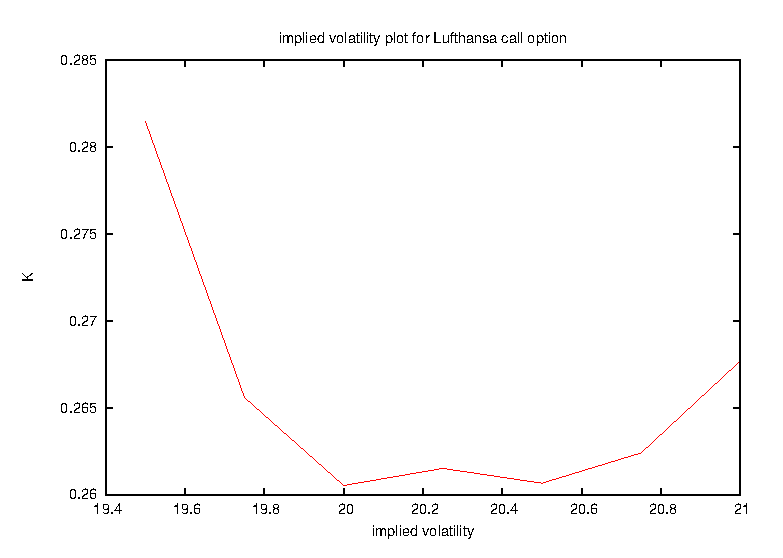
\includegraphics[width=.9\textwidth]{task9.eps}
\caption{volatility smile, Lufthansa call option}
\label{fig:Task9}
\end{figure}

\end{document}
